\documentclass[a4paper,norsk, 10pt]{article}
\usepackage[utf8]{inputenc}
\usepackage{verbatim}
\usepackage{listings}
\usepackage{graphicx}
\usepackage[norsk]{babel}
\usepackage{a4wide}
\usepackage{color}
\usepackage{amsmath}
\usepackage{float}
\usepackage{amssymb}
\usepackage[dvips]{epsfig}
\usepackage[toc,page]{appendix}
\usepackage[T1]{fontenc}
\usepackage{cite} % [2,3,4] --> [2--4]
\usepackage{shadow}
\usepackage{hyperref}
\usepackage{titling}
\usepackage{marvosym }
\usepackage{subcaption}
\usepackage[noabbrev]{cleveref}
\usepackage{cite}
\usepackage{todonotes}


\setlength{\droptitle}{-10em}   % This is your set screw

\setcounter{tocdepth}{2}

\lstset{language=c++}
\lstset{alsolanguage=[90]Fortran}
\lstset{alsolanguage=Python}
\lstset{basicstyle=\small}
\lstset{backgroundcolor=\color{white}}
\lstset{frame=single}
\lstset{stringstyle=\ttfamily}
\lstset{keywordstyle=\color{red}\bfseries}
\lstset{commentstyle=\itshape\color{blue}}
\lstset{showspaces=false}
\lstset{showstringspaces=false}
\lstset{showtabs=false}
\lstset{breaklines}
\title{AST5220 Milestone 2}
\author{Daniel Heinesen, daniehei}
\begin{document}
\maketitle
\section{Introduction}
In this exercise we are going to calculate the optical depth and visibility function. These quantities describe the how easy/difficult it is for a photon to travel. \todo{Rewrite} When later calculating the Boltzmann equations for the photons, we will have to use the optical depth \todo{And visibility function?}.

Due to the large amount of free electrons in the early Universe, photons could not travel far without being absorbed and scattered by the electrons. So to get a sense of the optical depth of the photons, we need to know the amount of electrons we have in our Universe. This will be done with the Saha and Peebles' equation. Having the density of electrons we can easily find the optical depth and visibility function. From these we can find out at which point the Universe was translucent enough for the photons to travel freely; this is the time of recombination.

\section{Theory}
We cannot find the electron density $n_e$ directly. We need to go through the fractional electron density $X_e = n_e/n_H$, where $n_H$ is the density of hydrogen in the Universe. To find $X_e$ we are going to use two different equations. If $X_e \approx 1$ -- meaning that there are way more free electrons than neutral \todo{Does $H$ mean neutral hydrogen} hydrogen in the Universe -- we can use the Saha equation
\begin{equation}\label{eq:saha}
\frac{X_e^2}{1-X_e} = \frac{1}{n_b}\left(\frac{m_e T_b k_b}{2\pi \hbar^2}\right)^{3/2} e^{-\epsilon_0/T_b k_b},
\end{equation}
where $n_b$ is the density of baryons, $m_e$ the mass of an electron and $T_b$ the temperature of the baryons. If we have $X_e < 0.99$ this equation becomes inaccurate and we need to solve Peebles' equation. This equation describes $X_e$ for all values of $X_e$ but is more difficult to solve, thus why be use the Saha equations for the earliest times. The Peebles' equation is given as
\begin{equation}\label{eq:peebles}
\frac{dX_e}{dx} = \frac{C_r}{H}\left[\beta (T_b)(1-X_e) - n_H \alpha^{(2)}(T_b)X_e^2 \right],
\end{equation}
where

\begin{equation}
C_r (T_b) = \frac{\Lambda_{2s \rightarrow 1s}+ \Lambda_{\alpha}}{\Lambda_{2s \rightarrow 1s} + \Lambda_{\alpha} + \beta^{(2)}(T_b)},
\end{equation}
\begin{equation}
\Lambda_{2s\rightarrow 1s} = 8.227 s^{-1},
\end{equation}
\begin{equation}
\Lambda_{\alpha} = \frac{H}{(\hbar c)^3}\frac{27\epsilon_0^3}{(8\pi)^2 n_{1s}},
\end{equation}
\begin{equation}
n_{1s} = (1-X_e)n_{H},
\end{equation}
\begin{equation}\label{eq:beta2}
\beta^{(2)}(T_b) = \beta(T_b)e^{3\epsilon_0/4T_bk_b},
\end{equation}
\begin{equation}\label{eq:beta}
\beta(T_b) = \alpha^{(2)}(T_b)\left(\frac{m_eT_b k_b}{2\pi \hbar^2}\right)^{3/2}e^{-\epsilon_0/T_bk_b},
\end{equation}
\begin{equation}
\alpha^{(2)}(T_b) = \frac{64\pi}{\sqrt{27\pi}}\frac{\alpha^2}{m_e^2}\sqrt{\frac{\epsilon_0}{T_bk_b}}\frac{\hbar^2}{c}\phi_{2}(T_b),
\end{equation}
\begin{equation}
\phi_{2}(T_b) = 0.448\ln(\epsilon_0/T_bk_b).
\end{equation}

All of these equation use SI units. 

From $X_e$ we can find

\begin{equation}\label{eq:n_e}
n_e = X_e n_H,
\end{equation}
where
\begin{equation}
n_H = n_b \approx \frac{\rho_b}{m_H} = \frac{\Omega_b \rho_c}{m_h a^3}.
\end{equation}
We can use this because we assume that all baryonic matter in the Universe is hydrogen.

With this one could find the optical depth, defined as 
\begin{equation}\label{eq:tau}
\tau(\eta) = \int_{\eta}^{\eta_0} n_e \sigma_T a c d\eta \Leftrightarrow \tau(x) = \int_x^{x_0 = 0} - \frac{n_e \sigma_T a c}{\mathcal{H}} dx,
\end{equation}
where $\sigma_T$ is the Thompson cross section, $c$ is the speed of light, $a$ is the scale factor, $x$ is the logarithm scale factor and $\mathcal{H}$ the scaled Hubble parameter $aH$. And finally from this we can get the visibility function

\begin{equation}\label{eq:g}
\tilde{g} (x) = -\tau'e^{-\tau} = -\frac{d\tau}{dx}e^{-\tau}.
\end{equation}


\section{Method}
To find all the quantities below we need to integrate over a time variable. We are here using the logarithmic scale factor $x = \ln a$. For the integrations we will set up a grid of $x$-values from $x = \ln 10^{-10} \approx -23$ to $0$, with $1000$ points.

\subsection{Finding $X_e$ and $n_e$}
We mentioned above, we can use two different methods to find $X_e$ for two different epochs: The Saha equation when $X_e \approx 1$, and Peebles' equation when $X_e < 0.99$. 

The Saha equation \eqref{eq:saha} is a normal quadratic equation, which we can write as

\begin{equation}
X_e^2 + X_e\cdot C - C = 0,
\end{equation}

where $C = \frac{1}{n_b}\left(\frac{m_e T_b k_b}{2\pi \hbar^2}\right)^{3/2} e^{-\epsilon_0/T_b k_b}$. This can be solved by the normal quadratic formula. But since this is an equation which can be a bit unstable \footnote{By this I mean that we can have a subtraction of two small numbers, which is numerically unstable}. So we will instead use a more stable solution

\begin{equation}
X_e = \frac{2c}{-b \mp \sqrt{b^2 - 4ac}} = \frac{-2C}{-C - \sqrt{C^2 + 4C}}.
\end{equation}
We only used the negative sign in the $\mp$ because this ensures us a positive $X_e$.

When $X_e$ goes below $0.99$ we will switch to Peebles' equation \eqref{eq:peebles}. This is a differential equation, so here we will use the same solver as in milestone1. This is a integration method, using the \textit{rkqs} integration scheme. There is some numerical instability in the integrand, with the two exponents in \eqref{eq:beta2} and \eqref{eq:beta} causing some problems. But if we combine them, they become stable. Also not that we will need to find $H$ for a given $x$, this is done with a function from milestone 1.

From $X_e$ we can now use \eqref{eq:n_e} to get $n_e$. Later we will have to get values of $n_e$ for any values of $x$. Since we found $n_e$ for only $1000$ different $x$-values, we need to spline $n_e$. This is done with an algorithm from \textit{Numerical Recipes}. \todo{Rewrite...}

\subsection{Finding $\tau$ and $\tilde{g}$}

Next step is to calculate $\tau (x)$ from \eqref{eq:tau}. This is straight forward except from the fact that we do not have an initial condition for the earliest $x$, instead we know that the optical depth today is $\tau(x_0) = 0$. This means that we will integrate \eqref{eq:tau} in reverse, starting at today, and integrating backwards in time. As with $n_e$, we will also make a spline of $\tau$. But we will also use a spline function to get the first derivatives $\tau'$, which will be useful later. We will also make a spline function of the second derivatives $\tau''$.

Having $\tau'$ we can calculate $\tilde{g}$ from \eqref{eq:g}. We will also use splines to get a continuous function for $\tilde{g}$, as well as $\tilde{g}'$ and $\tilde{g}''$.

\section{Results}

\begin{figure}[!htb]
\centering
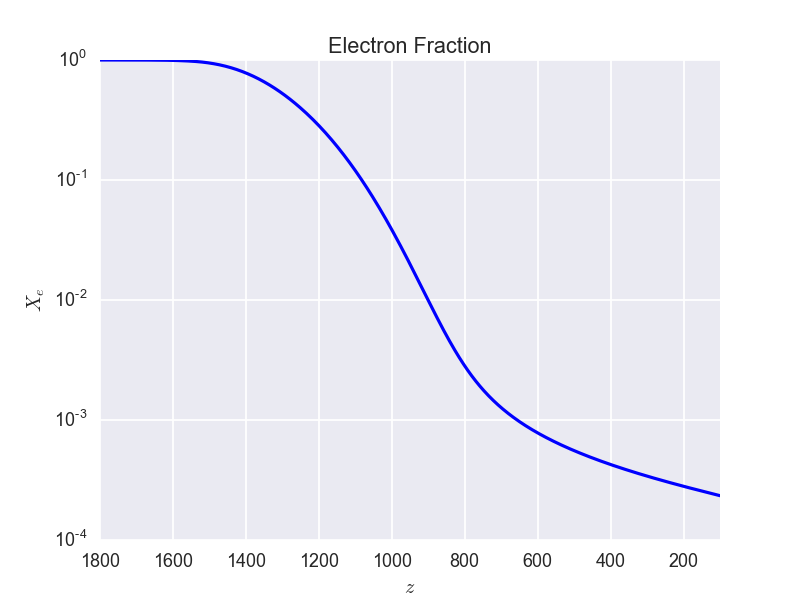
\includegraphics[scale=0.5]{xe.png}
\caption{Electron fraction $X_e$ as a function of red-shift $z$.}\label{fig:xe}
\end{figure}

Figure \ref{fig:xe} show the evolution of $X_e$. This figure starts at red-shift $z=1800$ which corresponds to $x\approx -7.5$. At about $z\approx 1500$, $x\approx -7.3$, we see that $X_e$ becomes smaller than $0.99$, meaning that we used the Saha equation for over half of the values $X_e$. Had we used Peebles' equation for every value of $x$, this calculation would had taken over double the time.

In the period $z = 1400$ to $z = 800$ we see a sharp decrease in the fraction of electrons in the Universe. During this period we say that recombination occurs.

\begin{figure}[!htb]
\centering
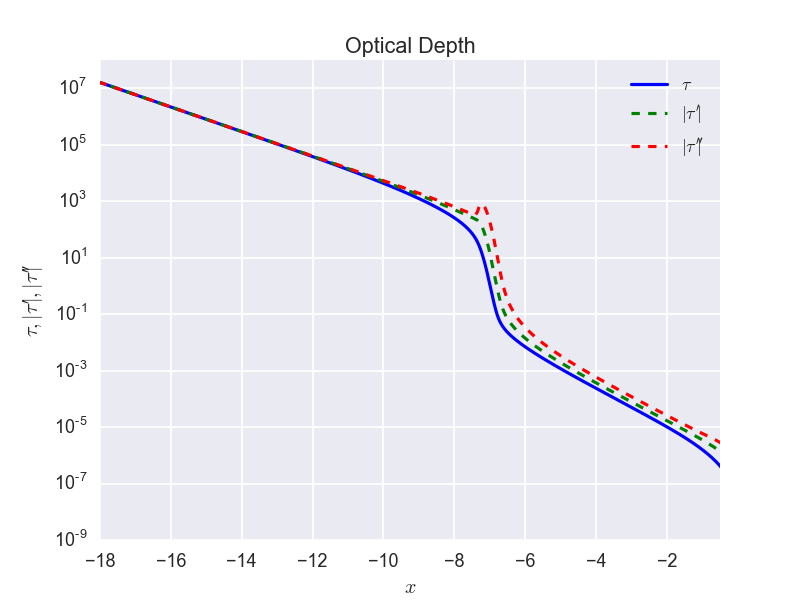
\includegraphics[scale=0.5]{tau.png}
\caption{Optical depth $\tau$, and its derivatives, as a function of the logarithmic scale factor $x$. To get all the variables in the same plot, a logarithmic y-axis is used.}\label{fig:tau}
\end{figure}

Figure \ref{fig:tau} shows that the optical depth steady decreases as more and more electrons are recombined with the protons to make hydrogen. But around $x\approx -7$, there is a sharp drop, which is not unlike the drop in $X_e$. Is, again, is the recombination. \todo{Write more (about the derivatives)}.

\begin{figure}[!htb]
\centering
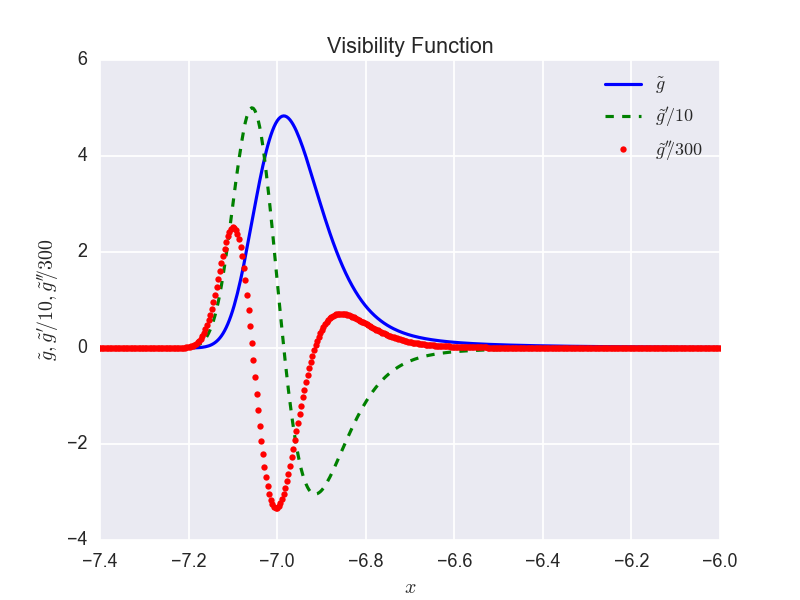
\includegraphics[scale=0.5]{g.png}
\caption{The visibility function $\tilde{g}$, and its scaled derivatives, as a function of $x$.}\label{fig:g}
\end{figure}

Figure \ref{fig:g} show the visibility function. Again we see that $\tilde{g}$, and its derivatives, are more or less constant throughout time, but around $x\approx -7$ there is a sudden change in all of the quantities. Once more indicating recombination.


\section{Discussion and Conclusion}
We have seen that for $X_e$, $\tau$ and $\tilde{g}$ there is something happening around $x\approx -7$. What is happening is that as the temperature in the Universe decreases, the primordial plasma and photons becomes colder. At a certain temperature the photons lacks the energy to tear the electrons and protons apart: Now they are free to recombine. Rapidly all the free electrons becomes apart of the neutral hydrogen atoms, leading $n_e$ to become smaller. This causes the rapid fall in the electron fraction $X_e$ we see in fig. \ref{fig:xe}.

In the earliest Universe, the photons and the free electrons are strongly interacting, meaning that a photon only travels for a short distance before being absorbed and scattered by an electron. This makes it impossible for the photon to travel freely, and the Universe is opaque. But as $X_e$ decreases, the photons becomes more free to travel further. This ability to travel freely is what the optical depth $\tau$ measure \todo{Is it?}: $\tau$ measures the opaqueness of the medium, the bigger $\tau$ is, the thicker the medium is, thus more opaque. This is why we see the sudden, 5-fold decrease in $\tau$ near $x\approx -7$: As the density of free electron fall, the photons can travel more freely and the opaqueness decreases.

Finally, the visibility function describes the probability that given a observed photon, it was last scattered at $x$, with the probability $\tilde{g}(x)$. Before recombination the Universe was opaque, so we do not expect the photon to be from this epoch. After recombination the Universe is more or less empty at larger scales, so the photons won't scatter of anything. So we expect that the last time the photons scattered was as recombination happened -- to exaggerate: In one instance the photons scattered of a bunch of free electrons, and in the next instance, the Universe was empty --. This is known as the last scattering. Looking at fig. \ref{fig:g} we see that it is most likely that an observed photon was scattered at $x\approx -7$, which means, once again, that this is where recombination happened.

So we now have continuous functions of $n_e$, $\tau$ and $\tilde{g}$ -- and their derivatives --, which will be used later when calculating the Einstein-Boltzmann equations. We also so that we could use these quantities to show that recombination happened around $x\approx -7$.





\end{document}

